%!TEX root = ED_Grafo.tex

\section{Coloração de Grafos}
\newcommand{\drawFilledNode}[4][1-]{%
	\node<#1>[circle,draw,fill,#2] at (#3) {\textcolor{black}{#4}};
}%

\begin{frame}[label=notas]
	\begin{block}{Coloração [de um Grafo]}
		Associação de uma cor a cada vértice do grafo de uma tal maneira que 
		dois vértices adjacentes não tenham a mesma cor.
	\end{block}
	\vfill\pause
	\begin{exampleblock}{Grafos Planares}
		Podem ser desenhados em um plano sem que duas arestas se cruzem.
	\end{exampleblock}
	% \pause
	% \begin{columns}
	% \column{.35\textwidth}
	%	\begin{itemize}
	%		\item[v] vértices
	%		\item[a] arestas
	%		\item[f] faces
	%	\end{itemize}
	% \column{.5\textwidth}
	%	A fórmula de Euler\footnote[frame]<2->{Uma árvore tem 1 face. Um cubo (vértice = canto) tem 6 faces.} diz que $$v-a+f=2$$
	% \end{columns}
	% \vfill
	% Um grafo planar tem, no máximo, $3v-6$ arestas (para $n > 2$).
	%Se toda face é limitada por, no mínimo, 3 arestas e cada aresta separa, no máximo, 2 faces, % 2a >= 3f
\end{frame}

\begin{frame}[label=notas]
	Um mapa de vários países desenhado em uma folha de papel, deve ser colorido 
	de modo que, para uma melhor visualização, dois países com uma fronteira em 
	comum devem ter cores distintas.  Qual é o número mínimo de cores exigidas 
	para a coloração de qualquer mapa?
	\\\vfill\pause
	\subitem{Associado a qualquer mapa existe um grafo, chamado o grafo dual do 
			  mapa}
	\vfill\pause
	\begin{block}{Número Cromático [de um Grafo]}
		\emph{Menor} número de cores necessárias para se obter uma coloração em 
		dado grafo.
	\end{block}
\end{frame}

\begin{frame}
	\begin{center}
		\includegraphics<1 | handout:0>[height=17\baselineskip]{brasil1}
		\includegraphics<2>[height=17\baselineskip]{brasil2}
		\includegraphics<3 | handout:0>[height=17\baselineskip]{brasil3}
	\end{center}
\end{frame}

\begin{frame}[label=notas]
	\begin{itemize}[<+->]
		\item Como não foi possível obter um mapa que exigisse mais de quatro 
		cores, uma conjectura foi formulada:
		\subitem{\emph{Quatro cores são suficientes para colorir qualquer mapa.}}
		\item Este problema permaneceu sem solução por mais de cem anos.
		\item Em 1976, Wolfgang Haken e Kenneth Appel (Universidade de Illinois) 
		demonstraram o teorema\footnote<4->[frame]{Até hoje ninguém conseguiu uma 
		demonstração do teorema que não recorra a um computador.}.
	\end{itemize}
	\vfill
	\uncover<5->{
		\begin{block}{Teorema das Quatro Cores}
			Dado um grafo planar, quatro cores são suficientes para colori-lo de 
			forma a que vrtices adjacentes não tenham a mesma cor.
		\end{block}}
\end{frame}

\begin{frame}[label=notas]
	\framesubtitle{\uncover<3->{As vezes bastam 3...}}
	
	\begin{center}
		\includegraphics<1 | handout:0>[width=.5\textwidth]{australia}

		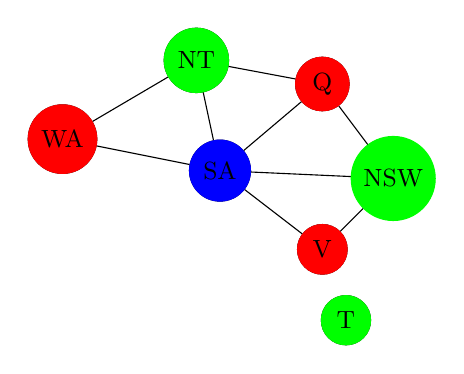
\begin{tikzpicture}[every node/.style={circle,draw}]
			\small
			\node<2> (WA) at (0, 0) {WA};
			\node<2> (NT) at (1.7, 1) {NT};
			\node<2> (SA) at (2, -0.4) {SA};
			\node<2> (Q) at (3.3, 0.7) {Q};
			\node<2> (NSW) at (4.2, -0.5) {NSQ};
			\node<2> (V) at (3.3, -1.4) {V};
			\node<2> (T) at (3.6, -2.3) {T};
			
			\draw<2-3> (SA) -- (WA) -- (NT) -- (Q) -- (NSW) -- (V);
			\draw<2-3> (SA) -- (NT);
			\draw<2-3> (SA) -- (Q);
			\draw<2-3> (SA) -- (NSW);
			\draw<2-3> (SA) -- (V);
			
			\node<3>[fill,red] at(WA) {\textcolor{black}{WA}};
			\node<3>[fill,green] at(NT) {\textcolor{black}{NT}};
			\node<3>[fill,blue] at(SA) {\textcolor{black}{SA}};
			\node<3>[fill,red] at(Q) {\textcolor{black}{Q}};
			\node<3>[fill,green] at(NSW) {\textcolor{black}{NSW}};
			\node<3>[fill,red] at(V) {\textcolor{black}{V}};
			\node<3>[fill,green] at(T) {\textcolor{black}{T}};
		\end{tikzpicture}
		\includegraphics<4 | handout:0>[width=.5\textwidth]{australia-solution}
	\end{center}
\end{frame}

\begin{frame}
	\framesubtitle{Contradição? \uncover<2->{Não...}}
	
\includegraphics[width=.45\textwidth]{Non-Counterexample_1}
	\hfill
	\includegraphics<2->[width=.45\textwidth]{Non-Counterexample_2}
\end{frame}

\begin{frame}[label=notas]
	Aplicações:
	\begin{itemize}
		\item Planejamento: tarefas conflitantes (que não podem ser realizadas ao mesmo tempo) são adjacentes.
		\vfill
		\item Alocação de Registros: recursos necessários ao mesmo tempo são adjacentes (otimização).
		\vfill
		\item Reconhecimento de padrões.
		\vfill
		\item Sudoku.
	\end{itemize}
\end{frame}